\documentclass[a4paper]{article}
\usepackage[utf8]{inputenc}
\usepackage{hyperref}
\usepackage{amsmath, amsfonts}
\usepackage{graphicx}

\newcommand{\agct}{{\usefont{OT1}{phv}{bc}{n}{AGCT}}}

\begin{document}
\title{Music processing for \agct{}}
\author{}
\date{\today}
\maketitle

This document tries to explain how we can use \href{https://github.com/agct2019/agct/}{\agct{}} to cluster music data. First, we present a high level overview of the process of clustering music data and then explain how the individual steps were implemented in more detail.

\section{Overview}
We will consider a fixed ``chunk'' of music and turn this into a high-dimensional vector to obtain one sample. This way we get many samples from one song. We can then input these samples, maybe together with samples from other songs, into \agct{} and apply clustering algorithms. We will use a neural network to analyze these ``chunks'' of music and turn them into a sample vector. The neural network will be some kind of autoencoder, where the extracted sample vector will just be the code vector.
To feed music data into the neural network, we first transform the track into a representation by tokens.

The entire process can be summarized as follows:
\begin{enumerate}
\item Extract the essential track (ie. melody-track)
\item Turn the music into a stream of tokens
\item Divide each song into smaller parts
\item Run each part through the autoencoder and extract the code vector.
\item Input the code vectors into \agct{} and run visualization and clustering algorithms.
\end{enumerate}

\begin{figure}[h!]
  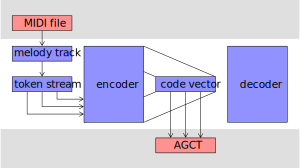
\includegraphics[width=\textwidth]{overview/process}
  \caption{Overview of the entire process. The decoder is only used to train the encoder.}
\end{figure}

To be able to analyze the music data on a per track (or even per note basis) we work with music files in MIDI file format. We also need to modify \agct{} a little, because there is currently no way to bypass the feature computation step.


\section{Implementation details}

We will first explain how \agct{} accepts raw coordinate inputs. Afterwards, we define the token representation of a music track. We then specify the model we used for the autoencoder and finally explain the training procedure (data and parameters).

\subsection{Using raw coordinates in \agct{}}
The first step was to make \agct{} accept raw coordinates. It was originally built to accept time series data, which will then go through a preprocessing step to extract the high-dimensional coordinates (eg. wavelet coordinates, slopes, \ldots). Optionally, one can chose to add an additional feature selection step, which allows to reduce the number of dimensions by keeping only the most significant coordinates.

\agct{} stores the data at multiple locations in memory, with different levels of processing. It is not entirely trivial to find out what data structures I have to be filled in to convince the program that it need not do any preprocessing but can instead go ahead at computing the manifold.

A great tip was to look at what preprocessing does in the case of using slopes and just mimic this behavior. This is what was eventually implemented: There is now a new preprocessing option that is just like slopes, except that it copies the data directly instead of computing any slopes.

The file format is exactly the same as before, but the time series are now interpreted as raw coordinates. In particular, you have to add a dummy time axis, which would otherwise denote the ``points in time'' when the data was measured. For example, the cube can be specified as follows:
\begin{verbatim}
Species
E (entity)	1	E1
EG (entity groupping)	1	1
T (time)	3	0	1 	2
R (replicate)	1
Data	8
V_000	-1	-1	-1
V_001	-1	-1	1
V_010	-1	1	-1
V_011	-1	1	1
V_100	1	-1	-1
V_101	1	-1	1
V_110	1	1	-1
V_111	1	1	1
\end{verbatim}

Note that there are 3 ``time measurements'', ie. 3 coordinates per data point. The three time stamps \texttt{1}, \texttt{2} and \texttt{3} were chosen completely arbitrary and do not carry any semantic meaning.

In general, there should be only one entity and only one entity group. The entity should belong to the first group (as there is only one group). As mentioned before, there has to be some kind of dummy time axis so that each dimension has one point in time associated to it. Replicate must be one. The number of data points can in principle be arbitrary. So can the name of a data point, as long as it does not interfere with string tokenization.

\begin{figure}[h!]
  \includegraphics[width=\textwidth]{agct/agct_all}
  \caption{Manifold and PCA display of geometric structures. The top row show the two dimensional sphere and the bottom row the two dimensional torus.}
\end{figure}

When loading a 2-dimensional manifold embedded into $\mathbb{R}^3$, the PCA tab usually gives a nice representation of it, while the manifold tab often looks distorted. Sometimes the Delaunay edges are missing. Occasionally, the clustering deadlocks, so the only option is to try again (It seems to happen more often with larger data). Also, scenarios most likely do not work with direct coordinates.

The version of \agct{} incorporating the changes described above was pushed to a new branch on the \href{https://github.com/agct2019/agct/}{repository of \agct{}} called \texttt{direct\_coordinates}. To load a file as raw coordinates, one just needs to select the ``Raw coordinates'' feature method (at the very bottom) when validating.

\subsection{Tokenizing a MIDI track}
To feed music into the autoencoder, we first have to make it sequential. Although music is inherently something sequential, an arbitrary number of notes can start, play or end at a given point in time, which makes it difficult to encode a time step with a fixed-sized vector. A good representation should be invariant under time shifts: A sequence of notes sound the same if they are at the beginning or at the end of a song. This means, we should use some kind of ``relative time'' instead of absolute time stamps. The token format we use was introduced in \cite{huang2018music}, but our version resembles more the one in use in \cite{topirceanu2014musenet}. MIDI files are processed using \href{https://salu133445.github.io/pypianoroll/index.html}{Pypianoroll} \cite{dong2018pypianoroll}.


\begin{figure}[h!]
  \includegraphics[width=\textwidth]{tokens/example}
  \begin{verbatim}
{
  "tick_duration": 0.01,
  "tokens": [
    [100,60], [0,50],
    [50,64], [0,50],
    [49,67], [0,50],
    [50,60], [50,64], [50,67], [50,72], [0,50]
  ]
}
  \end{verbatim}
  \caption{A pianoroll example and its representation in tokens, displayed as JSON format. The third note lasts for only 49 ticks, so that a new key-press is signaled at 1.5 seconds into the track. Also note the trailing time shift.}
  \label{tokens-example}
\end{figure}

The way a MIDI track is represented is illustrated in figure \ref{tokens-example}. It is represented as a floating point number, denoting the length of a tick (unit of time, 1/24 of a beat), together with a stream of tokens, specifying the actual notes. The stream of tokens contains two different types of tokens:
\begin{itemize}
\item Time shift tokens advance the current time (initially 0) by the number of ticks specified (integer).
\item Regular notes are encoded using two numbers: length and pitch. The (integer) length is the length of the note in number of ticks. The pitch is a value in $\{0, 1, \ldots, 127\}$, as obtained from the pianoroll matrix of \texttt{pypianoroll}. The start time of a note is always the current time.
\end{itemize}
A token \texttt{t} is a Python sequence type (tuple or list) containing exactly two non-negative integer values. In case of a time shift token, \texttt{t[0]} is zero and \texttt{t[1]} gives the number of ticks time is to be advanced. For note tokens, \texttt{t[0]} gives the length of the note and \texttt{t[1]} the pitch. Since the length of a note can never be 0, there will be no confusion between the two types of tokens. Incidentally, the zero token \texttt{[0, 0]} is a token that does nothing.

The stream of tokens may begin with a time shift token (in case of leading silence) and will always and with a time shift token that advances time until the end of the last note, or further in case of trailing silence. Hence the sum of all time shift tokens equals the length of the track. If multiple notes start at the same time, they are sorted in the stream of tokens with increasing pitch values. There are no consecutive time shift tokens and any two note tokens of the same pitch are separated by at least one tick. This makes the token representation unique.

Information about the program number or the intensity of a note (velocity) are not available in the tokenized format. Usually, a song consists of about approximately 2000 tokens.

\subsubsection{Converting to integers}

Tokens can be further converted into a natural number. We do this by first capping the length value of both types of tokens at 127. After this operation, all tokens conveniently live in the space $\{0, 1, \ldots, 127\}^2$. This allows us to convert the tokens to integers using a simple binary concatenation \begin{align*}
\{0, \ldots, 127\}^2 &\to \{0, \ldots, 16384\} \\
(l, p) &\mapsto l\cdot128+p.
\end{align*}
There reverse operation is (formally) just a simple modulo and division. This way the original token can be recovered, except that the lengths are capped at 127.

The threshold of 127 was somewhat arbitrary, but it leads to a more symmetric token space. Data suggests that the threshold value should be somewhere around 96 (or 4 beats) (see figure \ref{tokens-hist}), but 127 makes it the most simple.

\begin{figure}[h!]
  \includegraphics[width=\textwidth]{tokens/length}
  \caption{The length distribution of the two types of tokens.}
  \label{tokens-hist}
\end{figure}

\subsection{The Autoencoder}

We will use a model adapted from the \href{https://pytorch.org/tutorials/intermediate/seq2seq_translation_tutorial.html}{Seq2Seq tutorial} at PyTorch.\footnote{Since we want an unique code vector, we used the version without the attention.} The original idea stems from \cite{sutskever2014sequence}. Both the encoder and decoder consist of the same type of Recurrent Neural Network (RNN). We set the sequence length $n$ to a fixed value.

The encoder (see figure \ref{enc}) consists of an embedding layer and a gated recurrent unit (GRU). It receives as input a sequence of tokens in integer format as specified above. During each iteration, it embeds the current element of the sequence and feeds it through the GRU. The first hidden state vector $h_0$ was initialized to 0 and the last hidden vector $h_n$ is our code vector. Any other output from the GRU (ie. intermediate hidden vectors $h_i$ for $i\in\{0,\ldots,n-1\}$) is discarded.

\begin{figure}[h!]
  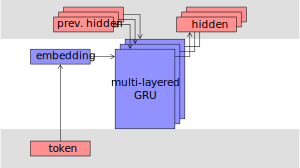
\includegraphics[width=\textwidth]{model/encoder}
  \caption{One iteration of the encoder. A new element of the sequence is processed by feeding its embedding together with the hidden vector produced by the previous element into the GRU.}
  \label{enc}
\end{figure}

The decoder contains an embedding, ReLU, GRU, linear and softmax layer. The decoder receives as input the last hidden vector of the encoder. During each iteration, it embeds the previous prediction and applies the ReLU function. The resulting value is then fed through the GRU together with the previous hidden vector. The output of the GRU is passed through the linear layer and finally softmax is applied. With \texttt{argmax}, the current prediction is then chosen. For the first iteration, the ``previous token'' was set to the \texttt{[0, 0]} token and the initial hidden vector of the decoder GRU is the code vector (ie. the last hidden vector of the encoder).
\begin{figure}[h!]
  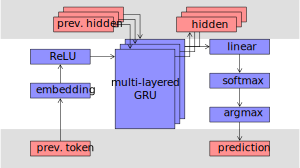
\includegraphics[width=\textwidth]{model/decoder}
  \caption{One iteration of the decoder. The linear layer turns the output of the GRU into a 16384-dimensional tensor, on which softmax can be applied to obtain the classification probabilities for each possible token. The one that is most likely is then chosen as the current prediction.}
  \label{dec}
\end{figure}

We further applied the following changes:
\begin{itemize}
\item According to \cite{sutskever2014sequence}, reversing the the input sequence improves accuracy, so we read the input sequence in reverse order.
\item The encoder and decoder share the embedding, so there is only one embedding.
\end{itemize}

\subsection{Training}
For training, we used the stochastic gradient descent (SGD) optimizer without momentum. We also decreased the learning rate by a constant multiplicative factor after every epoch. Since we do only very few epochs, the decrease in learning rate should be fairly significant.

\subsubsection{Dataset}
For training, we used a dataset derived from the \href{https://colinraffel.com/projects/lmd/}{Lakh MIDI Dataset}. More precisely, we used a subset of the \href{https://salu133445.github.io/lakh-pianoroll-dataset/dataset#lpd-5}{\texttt{lpd-5-cleansed}} dataset. \texttt{lpd-5-cleansed} contains 21425 pianorolls, where each MIDI-track is classified into one of the five categories \emph{Drums}, \emph{Piano}, \emph{Guitar}, \emph{Bass} and \emph{Strings}.

The first task was to identify the core part of a song, the melody track. Among all possible subsets, the aurally best result are obtained when retaining the piano and strings track, and removing the drums, guitar and bass tracks. However, this will lead to empty music files, when neither of piano and strings are present. These kind of tracks are ignored.\footnote{Another problem occurs when one of the two remaining tracks is accompaniment. The resulting music file has the tendency to over-emphasize the accompaniment, slightly obscuring the real melody. This is presumably due to the fact that information about velocity is lost during the conversion into tokenized format.} This leads to 9944 music files containing an average of 2131 tokens per song.

The individual sequences are then constructed using a sliding window. This way, a song of length $l$ gives rise to $l-n+1$ sequences of length $n$. In the end, we get for small sequence sizes (say, $n \leq 120$) approximately 20 million sequences, some of which look similar or might even the same.

\begin{figure}[h!]
  \includegraphics[width=\textwidth]{train/test-run}
  \caption{The training accuracy over 7 epochs. The learning rate was set to 0.001 and decreased by a factor of 0.6 after every epoch. Because of the random disconnects from Google Colaboratory due to time limits, we could only use the first 1000 songs to train.}
  \label{train-acc}
\end{figure}
 
\subsubsection{Teacher forcing}

Teacher forcing refers to the practice of feeding the correct element of the sequence back into the decoder even though it predicted the element incorrectly. Teacher forcing improves convergence speed, but introduces discrepancy between training and evaluation mode, which apparently leads to unstable predictions \cite{jaeger2002tutorial}. As motivated by \cite{bengio2015scheduled}, we start with a high teacher forcing ratio and linearly decrease it over time. We also flip a coin for each sequence element, instead of only once per sequence.\footnote{In case of mini-batches, the coin-toss result of one element is broadcast to all sequences in the batch.}

\bibliographystyle{plain}
\bibliography{refs}
\end{document}